An intitial mesh that satisfies LES surface resolution criteria in wall plus units at maximum Reynolds number is considered.
This mesh is referred to as M0\_nz50, where nz50 refers to the number of extruded layers in the spanwise/z direction.
As mentioned previously, mesh is refined in zones of high estimated error. 
Reduction in error can be seen as the mesh is refined in high error zones
The mesh details of all the meshes considered here as shown in Table \ref{table:adapt_mesh_details_Re200k}.

\begin{table}[H]
	\centering
	\caption{Summary of meshes for adaptive LES of $Re=200,000$ surging case}
	\label{table:adapt_mesh_details_Re200k}
	\begin{tabular}{|l|c|c|c|c|}
		\hline
		Mesh   & No. of elements \\
		\hline
		M0\_nz50	& 1,693,950 \\
		\hline
		Mza1\_nz50	& 4,758,800 \\
		\hline		
		Mza1\_nz100 & 9,517,600 \\
		\hline
		Mza2\_nz50  &  9,969,300 \\
		\hline
	\end{tabular}
\end{table}


\begin{figure}[H]
	\centering
	\begin{subfigure}[b]{0.475\textwidth}
		\centering
		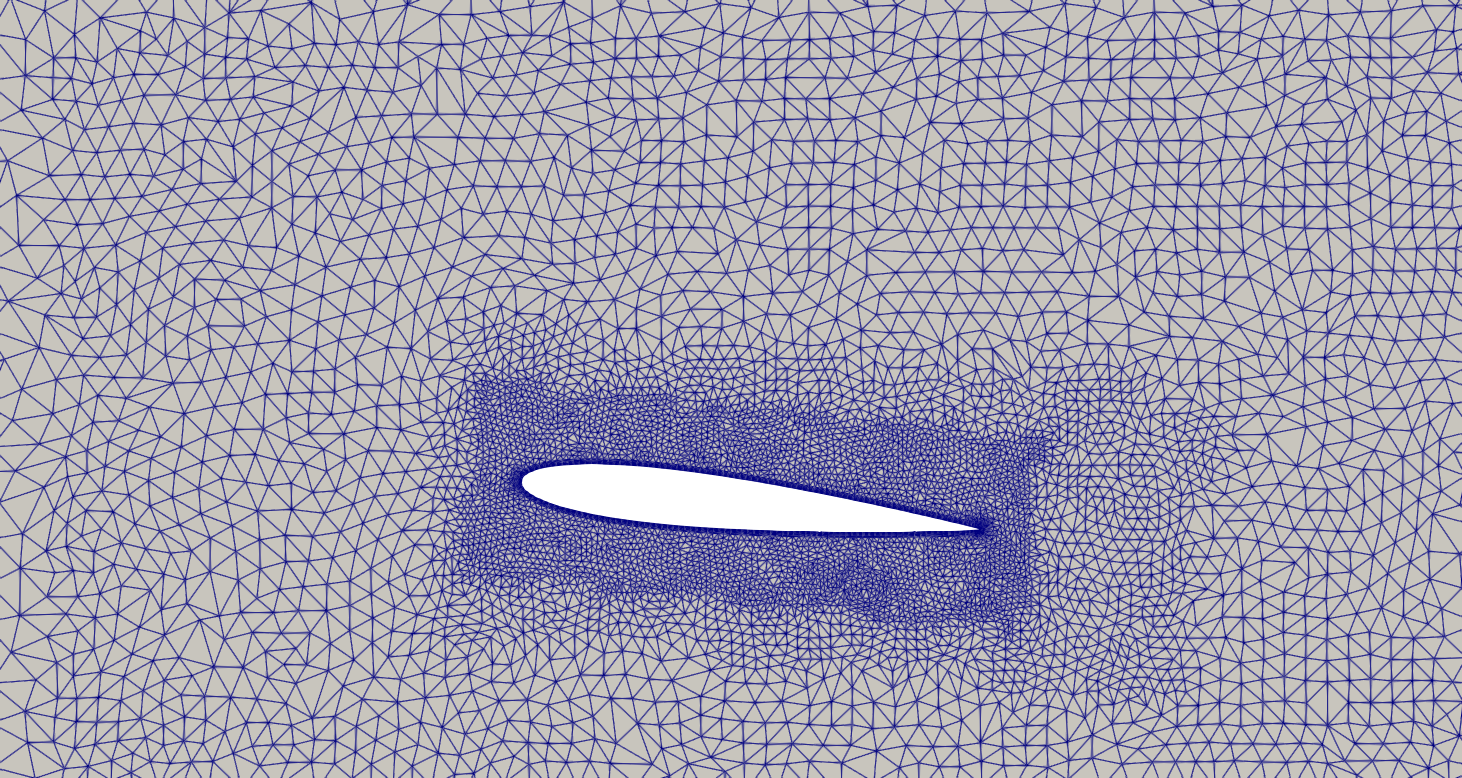
\includegraphics[width=1\textwidth]{figures/zonal_adapt_results/Mesh_and_error_plots_Re200k/M0_inplane.png}
		\caption{M0\_nz50 mesh}
		\label{fig:zonal_M0_mesh_Re200k}
	\end{subfigure}
	\begin{subfigure}[b]{0.475\textwidth}
		\centering
		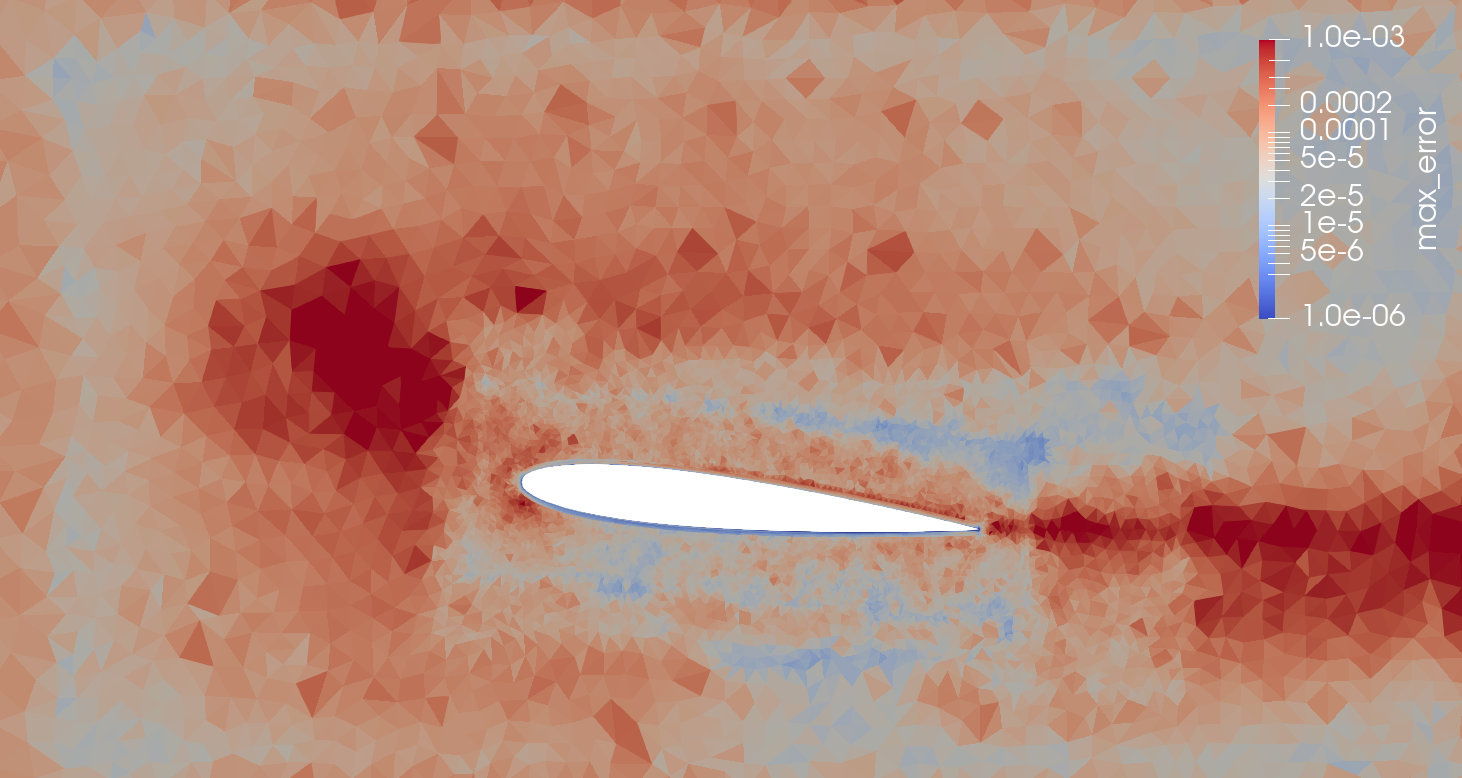
\includegraphics[width=1\textwidth]{figures/zonal_adapt_results/Mesh_and_error_plots_Re200k/M0_error.png}
		\caption{M0\_nz50 error field}
		\label{fig:zonal_M0_error_Re200k}
	\end{subfigure}
	
	\begin{subfigure}[b]{0.475\textwidth}
		\centering
		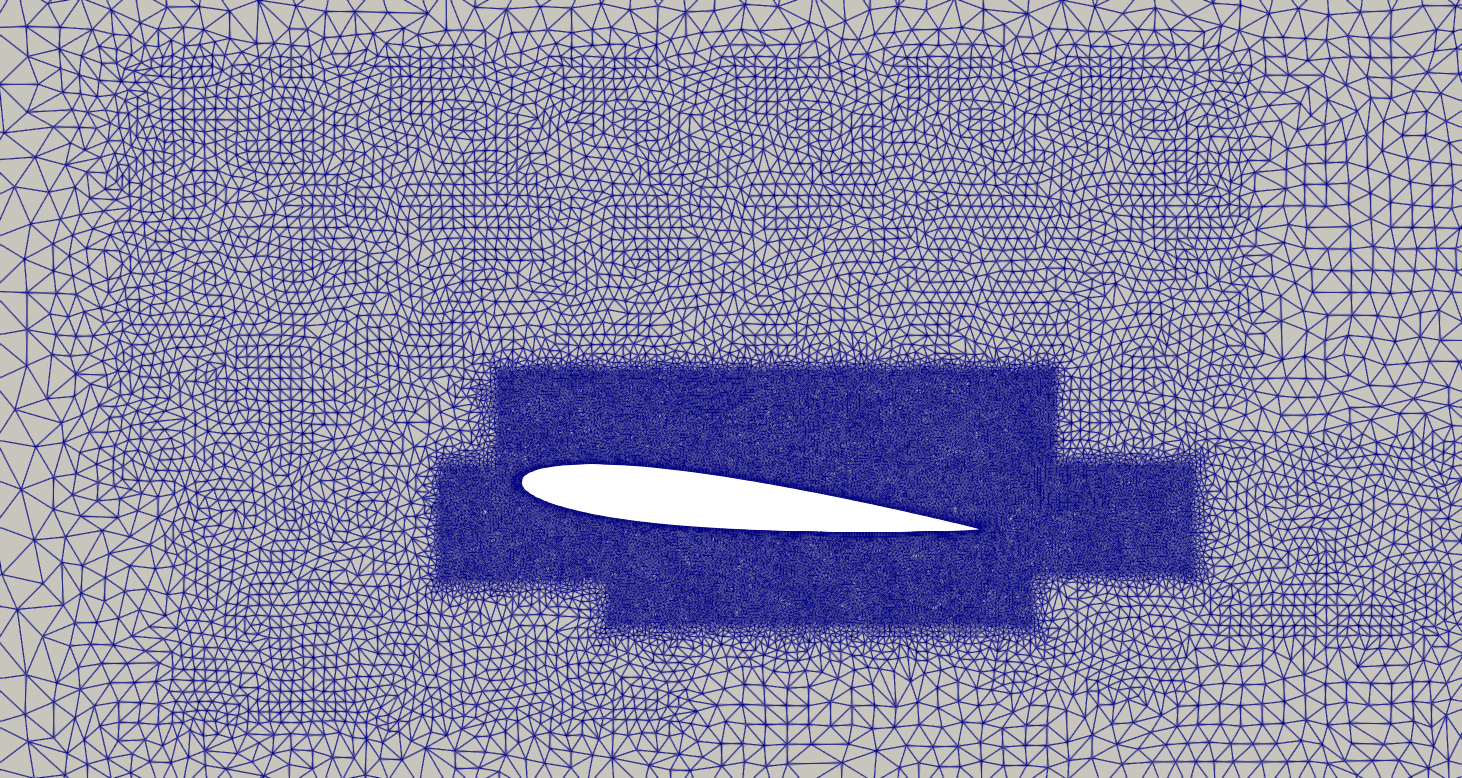
\includegraphics[width=1\textwidth]{figures/zonal_adapt_results/Mesh_and_error_plots_Re200k/Mza1_inplane.png}
		\caption{Mza1\_nz50 mesh}
		\label{fig:zonal_Mza1_mesh_Re200k}
	\end{subfigure}
	\begin{subfigure}[b]{0.475\textwidth}
		\centering
		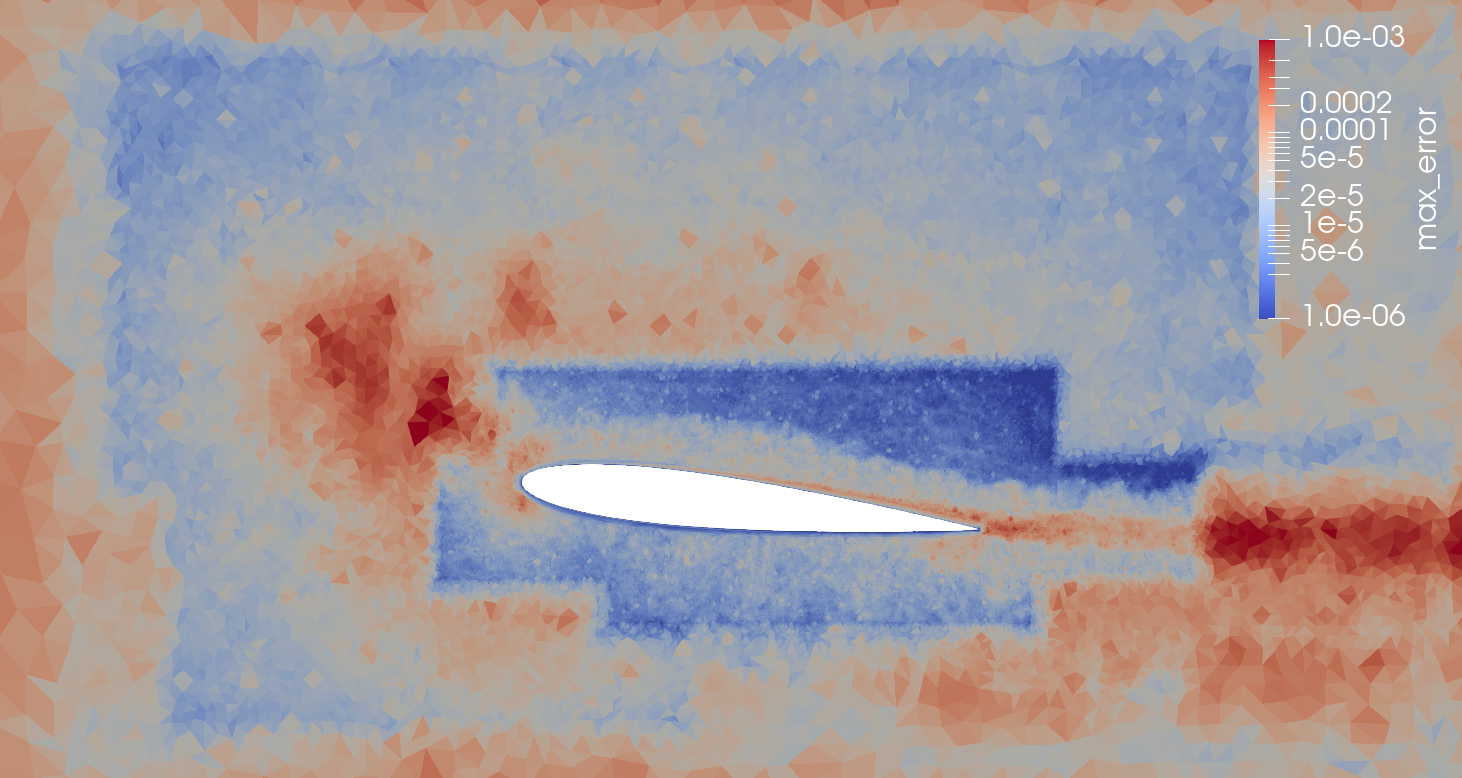
\includegraphics[width=1\textwidth]{figures/zonal_adapt_results/Mesh_and_error_plots_Re200k/Mza1_error.png}
		\caption{Mza1\_nz50 error field}
		\label{fig:zonal_Mza1_error_Re200k}
	\end{subfigure}
	
	
	\begin{subfigure}[b]{0.475\textwidth}
		\centering
		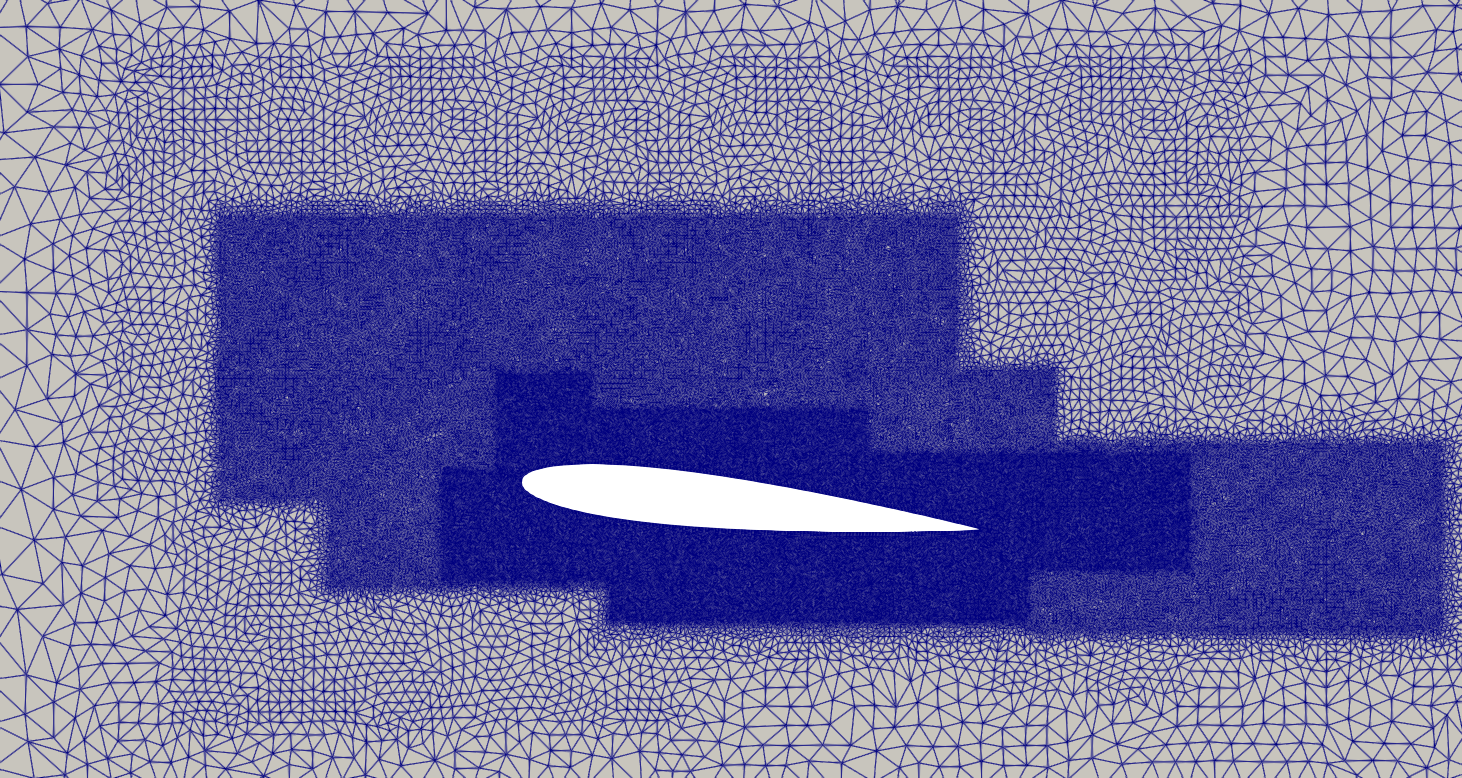
\includegraphics[width=1\textwidth]{figures/zonal_adapt_results/Mesh_and_error_plots_Re200k/Mza2_inplane.png}
		\caption{Mza2\_nz50 mesh}
		\label{fig:zonal_Mza2_mesh_Re200k}
	\end{subfigure}
	\begin{subfigure}[b]{0.475\textwidth}
		\centering
		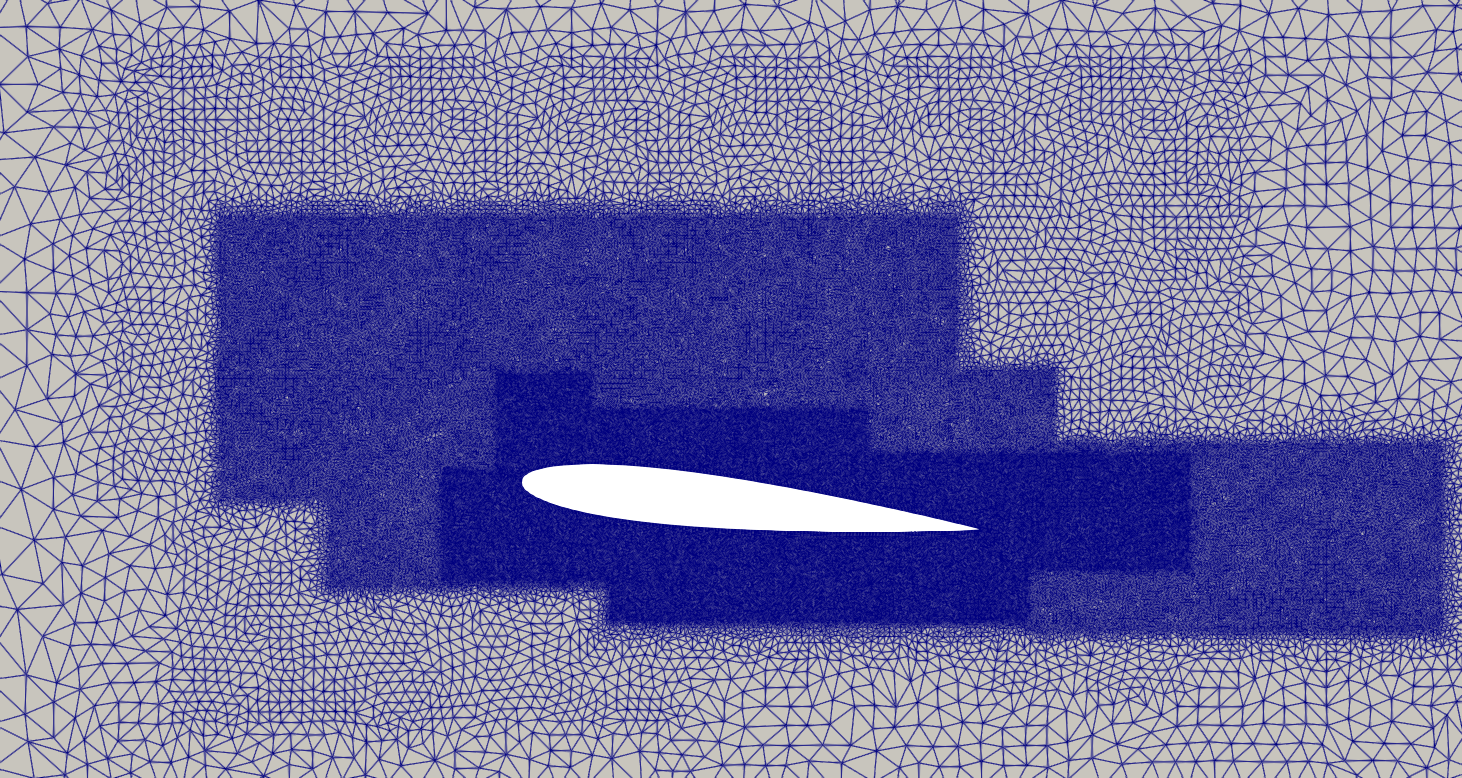
\includegraphics[width=1\textwidth]{figures/zonal_adapt_results/Mesh_and_error_plots_Re200k/Mza2_inplane.png}
		\caption{Mza2\_nz50 error field}
		\label{fig:zonal_Mza2_error_Re200k}
	\end{subfigure}
	
	\caption{Mesh and estimated error}
\end{figure}